\section{Observations \& Possible Paths}

\begin{frame}{Starting Point}
  \centering
    \color{Pink} Transfer Learning for DNN Applications for Constitutive Modeling \color{Black}
\begin{center}
  $\nabla \cdot \boldsymbol{\sigma} =0 \to  $ Equilibrium Equation 
\end{center}
 
\begin{minipage}{0.45\textwidth}
  \begin{block}{\color{White} Assumptions}
   \begin{itemize}
      \item Geometry 
      \item Material Model
   \end{itemize}
  \end{block} 
  \only<1> {
  \centering
    $\Downarrow$
  \begin{block}{\color{White} Parametrizations Examples}
   \begin{itemize}
      \item $V_f$, $L$
      \item $E$, $\nu$
   \end{itemize}
  \end{block}}
\end{minipage}%
\hspace{1cm}
\begin{minipage}{0.45\textwidth}
  \centering
  \begin{itemize}
      \item Learning objective: $\sigma=\mathcal{C}(\varepsilon, \cdot)$ 
  \end{itemize}
\end{minipage}
\end{frame}

\begin{frame}{Current ML-Mechanics Landscape}
\begin{minipage}{0.45\textwidth}
  \begin{block}{\color{White} Problems}<1-3>
    \begin{itemize}
      \item <3> Need of abundant data
      \item <3> Problem specific applications 
      \item <3> Single parameter considerations
    \end{itemize}
  \end{block} 
\end{minipage}%
\begin{minipage}{0.45\textwidth}
    \centering
    \color{Pink} \only<1>{Consider offline methods!} \only<2>{Why?}
  \end{minipage}
\end{frame}

\begin{frame}{Overarching Goal-A}
\centering
  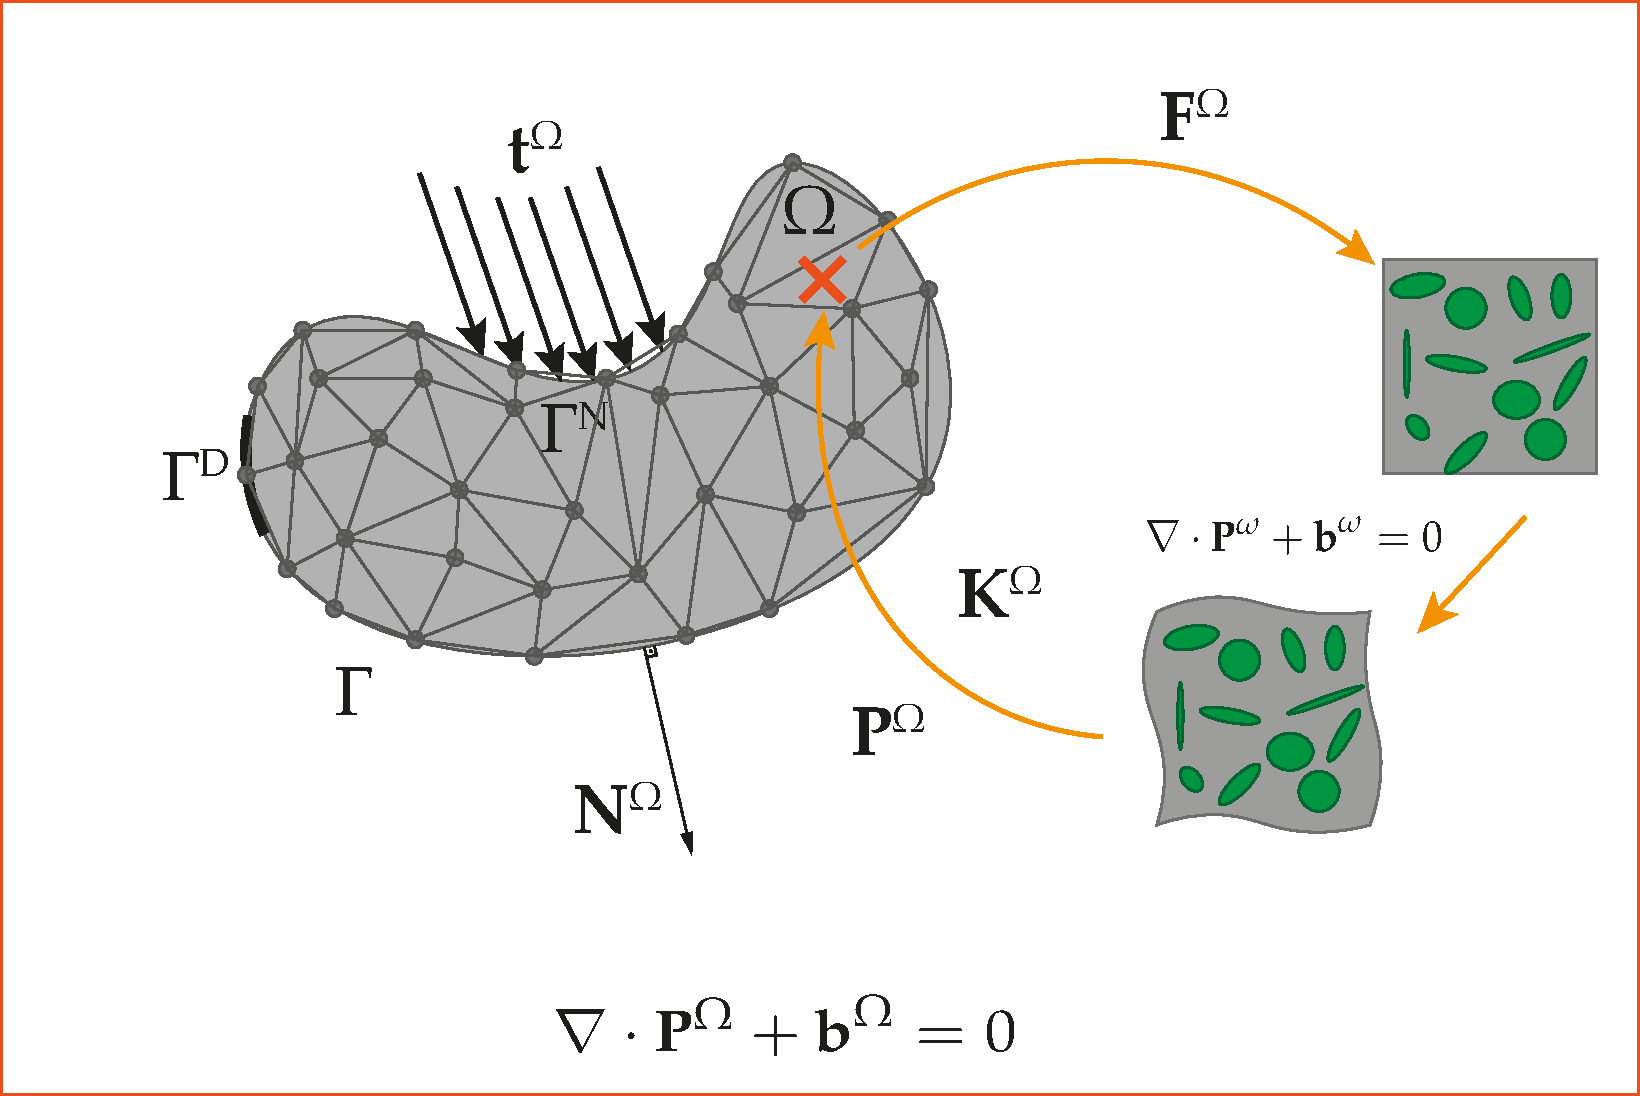
\includegraphics[width=0.45\textwidth]{Figures/myview/FE2-CONV}\hspace{1cm}\includegraphics[width=0.45\textwidth]{Figures/myview/fe2-ML}
\end{frame}

\begin{frame}{Overarching Goal-B}
\begin{minipage}{0.45\textwidth}
  \begin{block}{\color{White}Properties of $\mathcal{A}$}
  \begin{itemize}
    \item Capability to utilize past information
    \item Limited data demand 
    \item Good generalization 
  \end{itemize}
\end{block}
\end{minipage}%
  \begin{minipage}{0.5\textwidth}
    \centering
    \includegraphics[width=0.8\textwidth]{Figures/myview/fe2-ML}
  \end{minipage}
\end{frame}

\begin{frame}{Possible Paths}
  \begin{minipage}{0.6\textwidth}
    \begin{block}{\color{white}Access}
  \begin{itemize}
    \item<1> A parameterized oracle model for $\sigma=\mathcal{C}(\varepsilon, \cdot)$
  \end{itemize}
  \end{block}
  \begin{block}{\color{white}Possible Paths}
  \begin{itemize}
    \item<2> Learning the tasks space ($\sigma=\mathcal{C}(\varepsilon, \cdot))_{i=1}^M$
    \item<3> Effect of continual task observation...
    \item<4> Access to subspace of task as a whole 
    \item<5> Active sampling of tasks and data in a task
  \end{itemize}
  \end{block}
  \end{minipage}%
  \begin{minipage}{0.4\textwidth}
    \includegraphics<2-4>[width=\textwidth]{Figures/myview/tasks}
    \includegraphics<5>[width=\textwidth]{Figures/myview/task_space}
  \end{minipage}
\end{frame}

\begin{frame}{Holistic Problem}
\centering
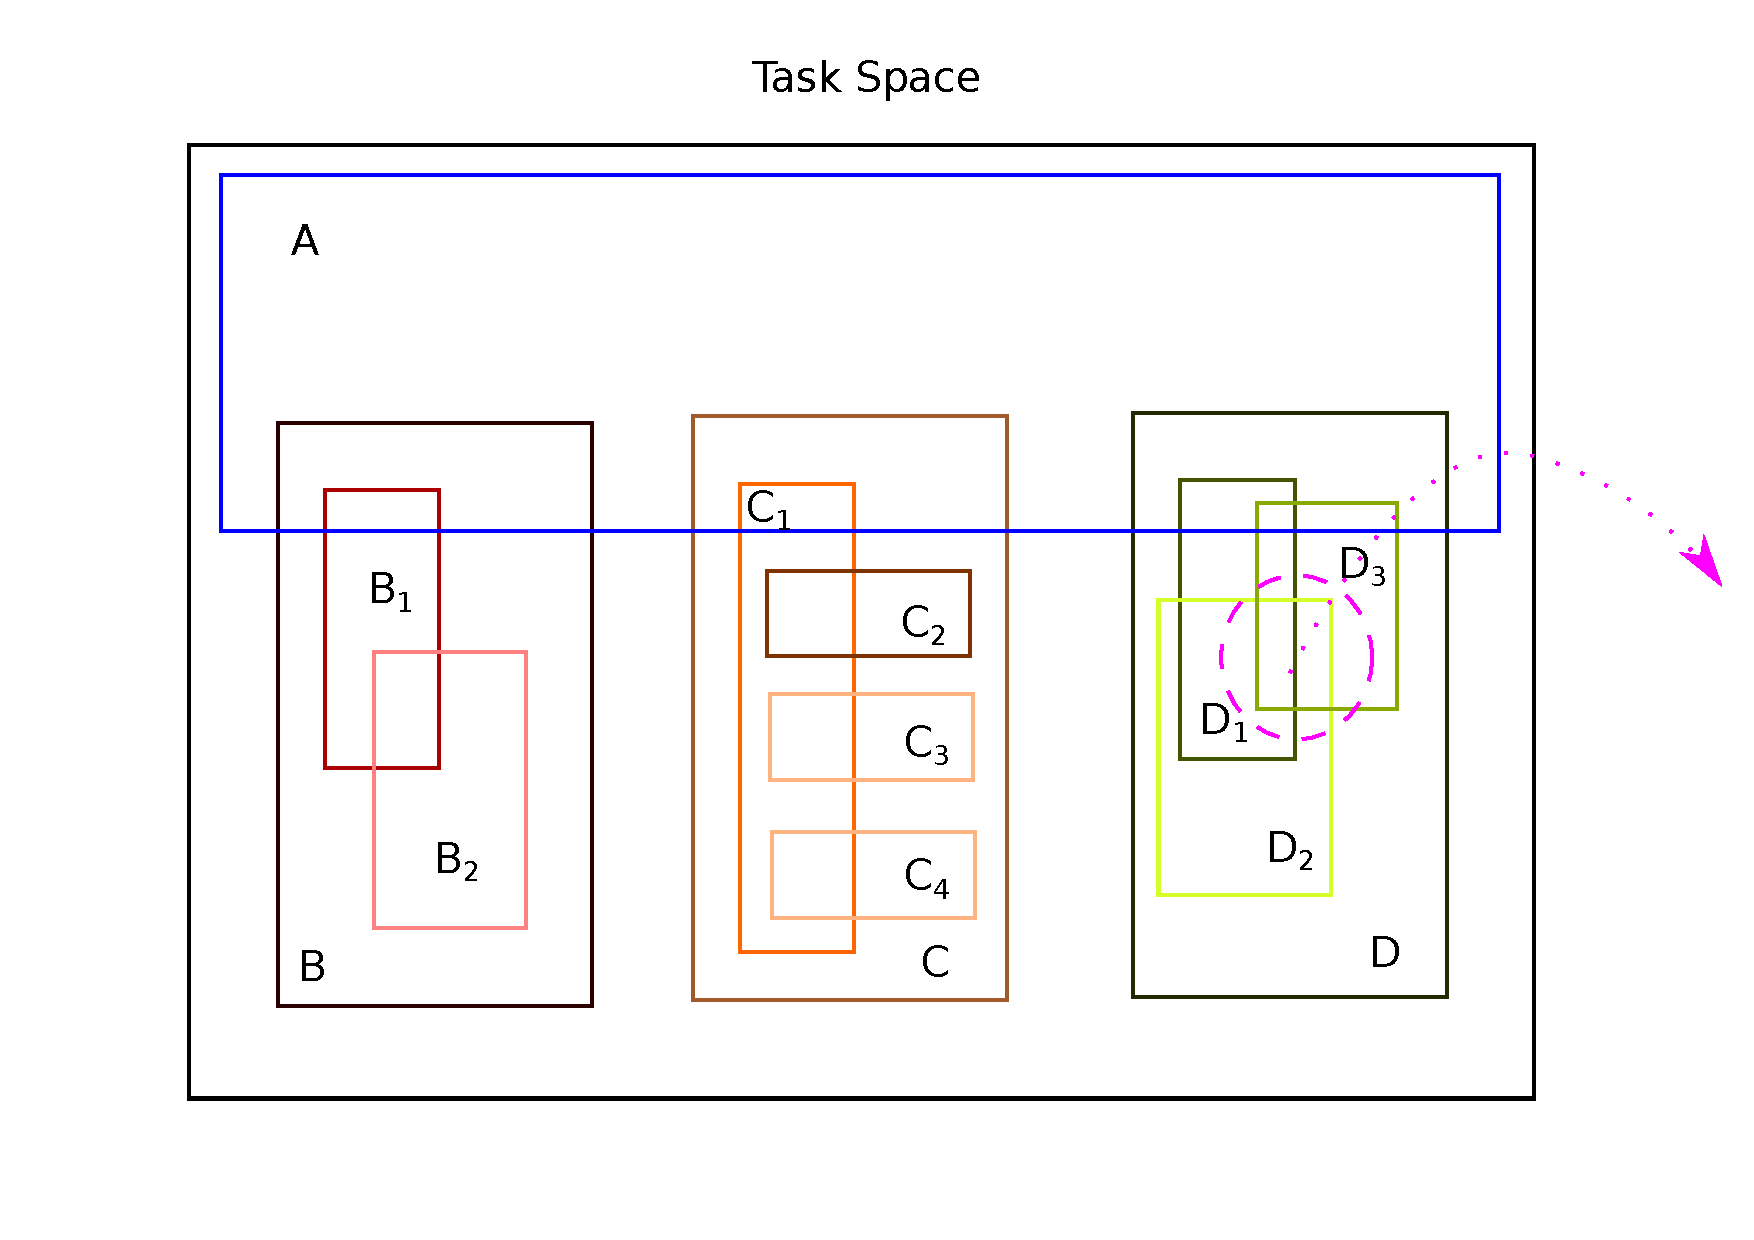
\includegraphics[width=0.6\textwidth]{Figures/myview/tasks.pdf}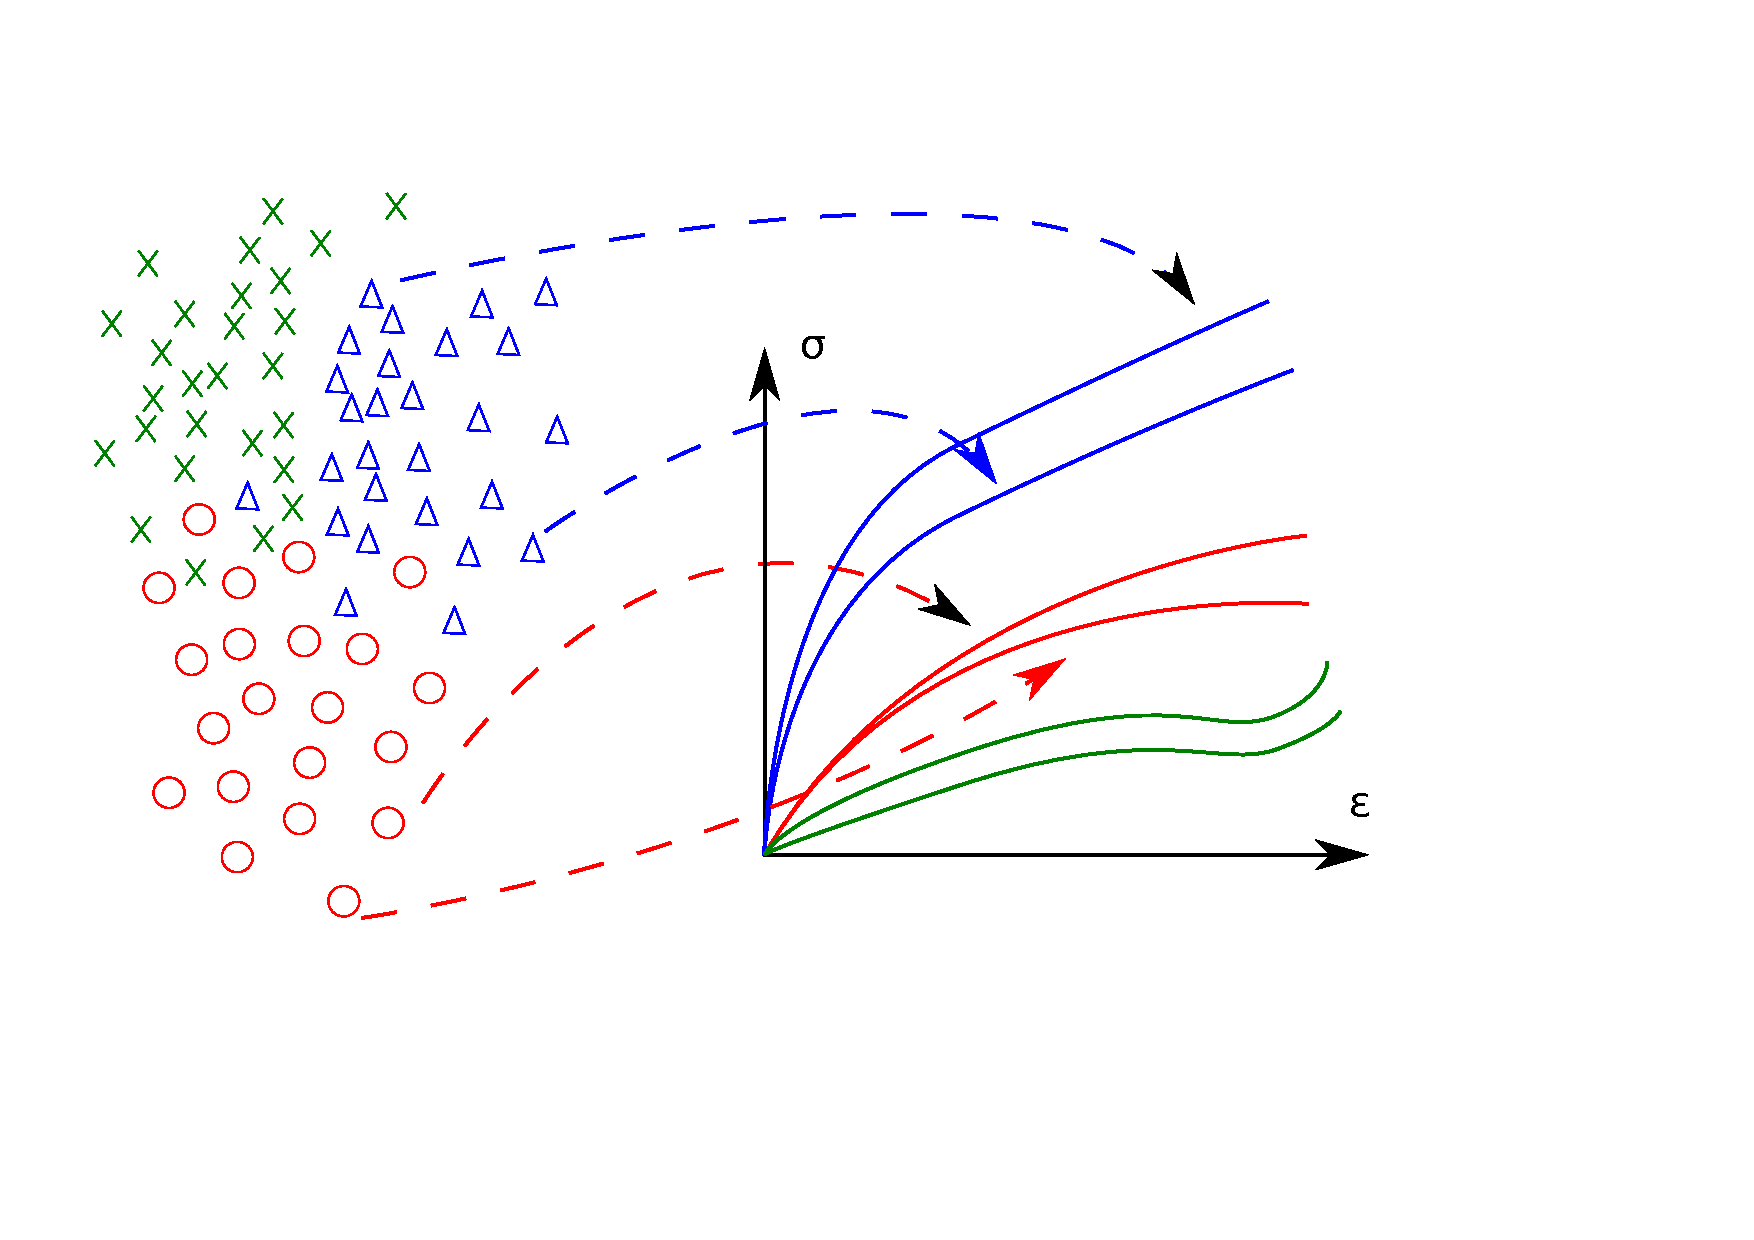
\includegraphics[width=0.4\textwidth]{Figures/myview/task_space.pdf}
\end{frame}

\begin{frame}{My work}
\centering
\begin{block}{\color{White} Until now}
  \begin{itemize}
    \item Data generation framework
  \end{itemize}
\end{block}
\begin{block}{\color{White} Currently}
  \begin{itemize}
    \item Generalization capabilities of MAML
  \end{itemize}
\end{block}
\begin{block}{\color{White} Future}
  \begin{itemize}
    \item Learning to Learn material models
    \item Domain adaptation and generalization if we consider the labels as full mappings?
  \end{itemize}
\end{block}
\end{frame}

\section{Summary}
\begin{frame}{Summary}
  \begin{itemize}
    \item Accelerate conventional PDE solution techniques (for certain problems)
    \item Learn $\sigma=\mathcal{C}(\varepsilon, \cdot)$ 
    \item Either past data or active sampling
  \end{itemize}
\end{frame}

